\documentclass[11pt]{article}
\frenchspacing
\usepackage{amsmath,amssymb,graphicx}
\usepackage[colorlinks=false,pdfborder={0 0 1}]{hyperref}
\usepackage[
    top=0.65in,
    bottom=0.65in,
    left=0.7in,
    right=0.7in
]{geometry}

\setlength{\parindent}{0pt}
\setlength{\parskip}{0.35em}

\begin{document}

\noindent
{\small Madison T. Hobbs}
\hfill
{\small MIT 16.S893, Assignment 2}

\vspace{0.25em}

\begin{center}
    {\normalsize \textbf{Reproduction of the Two-Phase Non-Charring Ablation Solution}}
\end{center}

\vspace{0.35em}

\section{Paper Objective and Reproduction Scope}
Ablative thermal protection removes energy by sacrificing material at a heated
surface. Numerical material-response codes can represent this process, but
they are difficult to verify when thermal conductivity, specific heat,
density, phase change, and surface recession are coupled. Kato and Matsuda
address this problem by deriving exact quasi-steady temperature relations for
a semi-infinite, one-dimensional, non-charring ablator with
temperature-dependent properties \cite{kato2022}. Their stated purpose is to
provide a rapid engineering estimate, clarify the behavior of the reduced
model, and supply a reference solution for checking numerical codes.

The paper treats a single-phase solid and a two-phase Teflon model. This
reproduction focuses on the two-phase model used in Figures~6 and 7. The model
contains an amorphous region next to the heated surface and a crystalline
region farther into the material. It includes surface recession, latent heat,
and different temperature-dependent properties in the two regions. It does
not include char formation or transport of pyrolysis gas.

Figure~6 compares the analytical profile with a finite-difference result for
one surface temperature and recession velocity. Figure~7 holds the recession
velocity fixed and varies the surface temperature. The reproduction evaluates
the analytical integrals, solves the original differential equation by two
independent numerical methods, checks physical properties and limiting cases,
and overlays the calculated curves on the published figures.

\section{Moving-Coordinate Energy Equation}
Let $y$ denote a stationary coordinate measured from the initial surface, and
let $S(t)$ be the recession distance. The coordinate fixed to the receding
surface is
\begin{equation}
 y=x+S(t),
 \qquad
 V=\frac{dS}{dt}.
 \label{eq:coordinate}
\end{equation}
The stationary one-dimensional heat equation is
\begin{equation}
 \rho(T)C_p(T)\left.\frac{\partial T}{\partial t}\right|_y
 =\frac{\partial}{\partial y}
 \left(k(T)\frac{\partial T}{\partial y}\right).
 \label{eq:stationary}
\end{equation}
At fixed $x$, the chain rule gives
\begin{equation}
 \left.\frac{\partial T}{\partial t}\right|_x
 =\left.\frac{\partial T}{\partial t}\right|_y
 +V\frac{\partial T}{\partial x}.
 \label{eq:chain}
\end{equation}
Because spatial derivatives in $x$ and $y$ are equal at a fixed time,
substitution of equation~\eqref{eq:chain} into equation~\eqref{eq:stationary}
gives
\begin{equation}
 \rho C_p\left.\frac{\partial T}{\partial t}\right|_x
 =\frac{\partial}{\partial x}
 \left(k\frac{\partial T}{\partial x}\right)
 +\rho C_pV\frac{\partial T}{\partial x}.
 \label{eq:transient-moving}
\end{equation}
The quasi-steady assumption sets the time derivative at fixed $x$ to zero, so
\begin{equation}
 \frac{d}{dx}\left(k(T)\frac{dT}{dx}\right)
 +V\rho(T)C_p(T)\frac{dT}{dx}=0.
 \label{eq:steady}
\end{equation}

Define the volumetric sensible-enthalpy difference from a reference
temperature $T_r$ as
\begin{equation}
 H(T;T_r)=\int_{T_r}^{T}\rho(u)C_p(u)\,du.
 \label{eq:enthalpy}
\end{equation}
Since $dH/dx=\rho C_p\,dT/dx$, equation~\eqref{eq:steady} can be written
\begin{equation}
 \frac{d}{dx}\left[k(T)\frac{dT}{dx}+VH(T;T_r)\right]=0.
\end{equation}
Its first integral is
\begin{equation}
 k(T)\frac{dT}{dx}+VH(T;T_r)=C.
 \label{eq:first-integral}
\end{equation}
The script \texttt{symbolic\_derivation.py} differentiates
\eqref{eq:first-integral} and verifies exact recovery of
\eqref{eq:steady}.

\section{Crystalline-Region Solution}
The local crystalline coordinate is $z=x-\delta_m$, where $\delta_m$ is the
amorphous-layer thickness. The crystalline boundary
conditions are
\begin{equation}
 T(0)=T_m,
 \qquad
 T(z)\rightarrow T_0,
 \qquad
 \frac{dT}{dz}\rightarrow0
 \quad\text{as}\quad z\rightarrow\infty.
 \label{eq:crystalline-bc}
\end{equation}
Taking $T_r=T_0$ in equation~\eqref{eq:first-integral} and applying the
far-field conditions makes $C=0$. Therefore,
\begin{equation}
 k_c(T)\frac{dT}{dz}
 =-V\int_{T_0}^{T}\rho_c(u)C_{p,c}(u)\,du.
 \label{eq:crystalline-gradient}
\end{equation}
Separating variables and integrating from $T$ to $T_m$ gives
\begin{equation}
 z(T)=\frac{1}{V}\int_T^{T_m}
 \frac{k_c(v)}{\displaystyle\int_{T_0}^{v}
 \rho_c(u)C_{p,c}(u)\,du}\,dv.
 \label{eq:crystalline-depth}
\end{equation}
The crystalline depth in the global coordinate is
\begin{equation}
 x(T)=\delta_m+z(T).
 \label{eq:crystalline-global}
\end{equation}
The inward conductive heat flux is defined as
$q=-k\,dT/dx$. Equation~\eqref{eq:crystalline-gradient} therefore gives
\begin{equation}
 q_c(T)=V\int_{T_0}^{T}\rho_c(u)C_{p,c}(u)\,du.
 \label{eq:crystalline-flux}
\end{equation}

\section{Amorphous Region and Phase Interface}
The amorphous boundary conditions are
\begin{equation}
 T(0)=T_s,
 \qquad
 T(\delta_m)=T_m.
 \label{eq:amorphous-bc}
\end{equation}
Define the crystalline sensible-energy contribution and phase-change
contribution as
\begin{equation}
 \phi_1=\int_{T_0}^{T_m}\rho_c(u)C_{p,c}(u)\,du,
 \qquad
 \phi_2=\rho_mh_m,
 \label{eq:phi}
\end{equation}
where the interface density used by the paper is
\begin{equation}
 \rho_m=\frac{\rho_a(T_m)+\rho_c(T_m)}{2}.
 \label{eq:interface-density}
\end{equation}
Conservation of energy across the moving phase interface requires
\begin{equation}
 q_a(T_m)-q_c(T_m)=V\rho_mh_m=V\phi_2.
 \label{eq:flux-jump}
\end{equation}
The amorphous heat flux that satisfies this jump is
\begin{equation}
 q_a(T)=V\left[
 \int_{T_m}^{T}\rho_a(u)C_{p,a}(u)\,du+\phi_1+\phi_2
 \right].
 \label{eq:amorphous-flux}
\end{equation}
Using $q_a=-k_a\,dT/dx$ and separating variables gives
\begin{equation}
 x(T)=\frac{1}{V}\int_T^{T_s}
 \frac{k_a(v)}{\displaystyle
 \int_{T_m}^{v}\rho_a(u)C_{p,a}(u)\,du+\phi_1+\phi_2}\,dv.
 \label{eq:amorphous-depth}
\end{equation}
The layer thickness follows directly from the temperature at the interface,
\begin{equation}
 \delta_m=x(T_m)
 =\frac{1}{V}\int_{T_m}^{T_s}
 \frac{k_a(v)}{\displaystyle
 \int_{T_m}^{v}\rho_a(u)C_{p,a}(u)\,du+\phi_1+\phi_2}\,dv.
 \label{eq:delta}
\end{equation}
Equations~\eqref{eq:amorphous-depth}, \eqref{eq:delta}, and
\eqref{eq:crystalline-global} define the full two-phase temperature profile.
The calculation first evaluates depth as a function of temperature, which is
monotone, and then numerically inverts that relation to obtain $T(x)$.

\section{Polynomial Evaluation and Scaling}
The published property fits are low-degree polynomials. If
\begin{equation}
 \rho(T)=\sum_i\rho_iT^i,
 \qquad
 C_p(T)=\sum_jc_jT^j,
\end{equation}
then
\begin{equation}
 \rho(T)C_p(T)=\sum_na_nT^n,
 \qquad
 a_n=\sum_{i+j=n}\rho_ic_j.
\end{equation}
The inner enthalpy integral is evaluated exactly as
\begin{equation}
 H(T;T_r)=\sum_n\frac{a_n}{n+1}
 \left(T^{n+1}-T_r^{n+1}\right).
 \label{eq:polynomial-enthalpy}
\end{equation}
The code forms these coefficients by polynomial convolution. Numerical
quadrature is only used for the remaining outer depth integral.

Both depth relations have the form $x(T)=F(T)/V$. Therefore,
\begin{equation}
 x(T;\lambda V)=\frac{x(T;V)}{\lambda},
 \qquad
 T(x;\lambda V)=T(\lambda x;V).
 \label{eq:velocity-scaling}
\end{equation}
This scaling supplies a test that does not depend on a digitized reference
curve.

\section{Material Properties and Figure 6 Conditions}
Figure~6 uses
\begin{equation}
 T_s=950\ \mathrm{K},\quad
 T_m=600\ \mathrm{K},\quad
 T_0=300\ \mathrm{K},\quad
 V=7.5545\times10^{-5}\ \mathrm{m/s},\quad
 h_m=58615\ \mathrm{J/kg}.
 \label{eq:figure6-conditions}
\end{equation}
The amorphous properties are
\begin{align}
 k_a(T)&=0.88090-0.0013984T+5.8197\times10^{-7}T^2,\\
 C_{p,a}(T)&=904.35+0.65314T,\\
 \rho_a(T)&=2070-0.7T,
 \label{eq:amorphous-properties}
\end{align}
and the crystalline properties are
\begin{align}
 k_c(T)&=0.050242+0.00061420T,\\
 C_{p,c}(T)&=514.98+1.5629T,\\
 \rho_c(T)&=2119+0.792T-2.105\times10^{-3}T^2.
 \label{eq:crystalline-properties}
\end{align}
SI units are used throughout. Substitution into equation~\eqref{eq:delta}
gives
\begin{equation}
 \delta_m=0.637199\ \mathrm{mm}.
 \label{eq:computed-delta}
\end{equation}
The paper reports $0.64\ \mathrm{mm}$. Since that value is rounded, the small
difference is not treated as a measured model error.

Figure~6 plots the piecewise profile
\begin{equation}
 T(x)=
 \begin{cases}
  T_a(x), & 0\leq x\leq\delta_m,\\
  T_c(x-\delta_m), & x>\delta_m,
 \end{cases}
 \label{eq:piecewise-profile}
\end{equation}
where $T_a$ and $T_c$ are the inverses of equations
\eqref{eq:amorphous-depth} and \eqref{eq:crystalline-depth}. The change in
slope at $T_m$ follows from the different material properties and the latent
heat term in equation~\eqref{eq:flux-jump}.

\section{Independent Numerical Calculations}
The first independent calculation applies a conservative finite-difference
form of equation~\eqref{eq:steady}. At an interior node,
\begin{equation}
 \frac{k_{i+1/2}(T_{i+1}-T_i)-k_{i-1/2}(T_i-T_{i-1})}{\Delta x^2}
 +(\rho C_p)_iV\frac{T_{i+1}-T_{i-1}}{2\Delta x}=0,
 \label{eq:finite-difference}
\end{equation}
where $k_{i+1/2}=(k_i+k_{i+1})/2$. This residual uses the differential
equation rather than the analytical temperature profile. The crystalline
domain is truncated at the paper's $L_\infty=0.05\ \mathrm{m}$.

The second independent calculation writes
\begin{equation}
 G=k(T)\frac{dT}{dx}
\end{equation}
and solves the first-order boundary-value system
\begin{align}
 \frac{dT}{dx}&=\frac{G}{k(T)},\\
 \frac{dG}{dx}&=-\rho(T)C_p(T)V\frac{G}{k(T)}.
 \label{eq:bvp-system}
\end{align}
Adaptive collocation is run with a requested tolerance of $10^{-8}$. This
provides a tighter numerical comparison than the fixed finite-difference grid
while remaining separate from the analytical quadrature and inversion.

\section{Symbolic and Test-Driven Verification}
The SymPy calculation checks three exact identities. It differentiates the
first integral to recover equation~\eqref{eq:steady}, reduces the phase-interface
energy residual to zero, and differentiates equation~\eqref{eq:polynomial-enthalpy}
to recover $\rho(T)C_p(T)$. These are algebraic checks and do not use floating
point tolerances.

Development followed short red--green--refactor steps. The first tests required
positive material properties and the published boundary conditions. Later
tests added the interface heat-flux jump, the reported layer thickness, the
constant-property limit, and the scaling in equation~\eqref{eq:velocity-scaling}.
The finite-difference and boundary-value calculations were then added as
independent references. Figure~7 ordering, plot generation, and paper overlays
were tested last.

The tests remain separated by purpose in \texttt{tests/}: material properties,
analytical behavior, energy balance, limiting behavior, independent numerical
solutions, error metrics, symbolic identities, and generated figures.

\section{Figure 7 Surface-Temperature Sweep}
Figure~7 uses the same properties, $T_m$, $T_0$, and $V$, but evaluates the
solution at
\begin{equation}
 T_s\in\{900,950,1000\}\ \mathrm{K}.
\end{equation}
For each surface temperature, equation~\eqref{eq:delta} determines a different
amorphous-layer thickness:
\begin{center}
\begin{tabular}{c|c}
$T_s$ (K) & $\delta_m$ (mm) \\
\hline
900  & 0.600428 \\
950  & 0.637199 \\
1000 & 0.665689
\end{tabular}
\end{center}
Increasing $T_s$ extends the amorphous integral over a larger temperature
interval and increases $\delta_m$. The crystalline relation $T_c(z)$ is
unchanged because $T_m$, $T_0$, $V$, and the crystalline properties are fixed.
Only its origin shifts in the global coordinate through
$x=\delta_m+z$. Figure~7 therefore checks both the predicted surface-temperature
trend and the translation of the crystalline profile.

\section{Verification and Error Metrics}
In the constant-property, single-phase limit, the solution reduces to
\begin{equation}
 T-T_0=(T_s-T_0)\exp\left(-\frac{V\rho C_p}{k}x\right),
 \label{eq:constant-limit}
\end{equation}
and a round-trip test recovers $x$ from the calculated temperature.

For numerical temperatures $T_i^{(n)}$ and analytical temperatures
$T_i^{(a)}$ at $N=501$ uniformly spaced depths, define
\begin{align}
 e_i&=T_i^{(n)}-T_i^{(a)},\\
 E_{\max}&=\max_i|e_i|,\\
 E_{\mathrm{RMSE}}&=
 \left(\frac{1}{N}\sum_{i=1}^{N}e_i^2\right)^{1/2},\\
 E_{\mathrm{rel}}&=100\max_i
 \left|\frac{e_i}{T_i^{(a)}}\right|,\\
 E_{\mathrm{NRMSE}}&=
 100\frac{E_{\mathrm{RMSE}}}
 {\max_iT_i^{(a)}-\min_iT_i^{(a)}}.
 \label{eq:error-measures}
\end{align}
The comparisons are calculated from temperature values rather than extracted
from image pixels.

\begin{center}
\begin{tabular}{c|r|r|r|r}
Case & FD max (K) & FD RMSE (K) & FD max (\%) & BVP max (K) \\
\hline
Fig. 6, 950 K  & 0.07535 & 0.00813 & 0.00818 & $8.6\times10^{-9}$ \\
Fig. 7, 900 K  & 0.04998 & 0.00881 & 0.00558 & $5.0\times10^{-9}$ \\
Fig. 7, 950 K  & 0.09244 & 0.01223 & 0.00979 & $4.9\times10^{-9}$ \\
Fig. 7, 1000 K & 0.15848 & 0.01898 & 0.01597 & $4.8\times10^{-9}$
\end{tabular}
\end{center}
The boundary-value calculation is tested with a
$2\times10^{-8}\ \mathrm{K}$ maximum-error limit. A $10^{-14}$ limit would be
reasonable for two equivalent algebraic expressions evaluated in double
precision, but not for a differential-equation solve requested at a
$10^{-8}$ tolerance.

\section{Interpretation and Limitations}
Figure~6 shows a monotone temperature decrease through both phases. The slope
changes at $T_m$ because the properties change and the interface consumes
latent heat. The analytical, finite-difference, and boundary-value profiles
agree across the plotted domain. Figure~7 shows that increasing $T_s$ raises
the profile and increases $\delta_m$; the curves become closer farther into
the crystalline material.

The model assumes one-dimensional conduction, a semi-infinite material,
constant $T_s$ and $V$, quasi-steady response, no thermal expansion, and a
fixed phase-transition temperature. It does not solve the external surface
energy balance, form char, or transport pyrolysis gas. The tests verify the
stated reduced model, not these assumptions for a particular flight or test
environment.

\begin{figure}[htbp]
 \centering
 \begin{minipage}{0.49\linewidth}
  \centering
  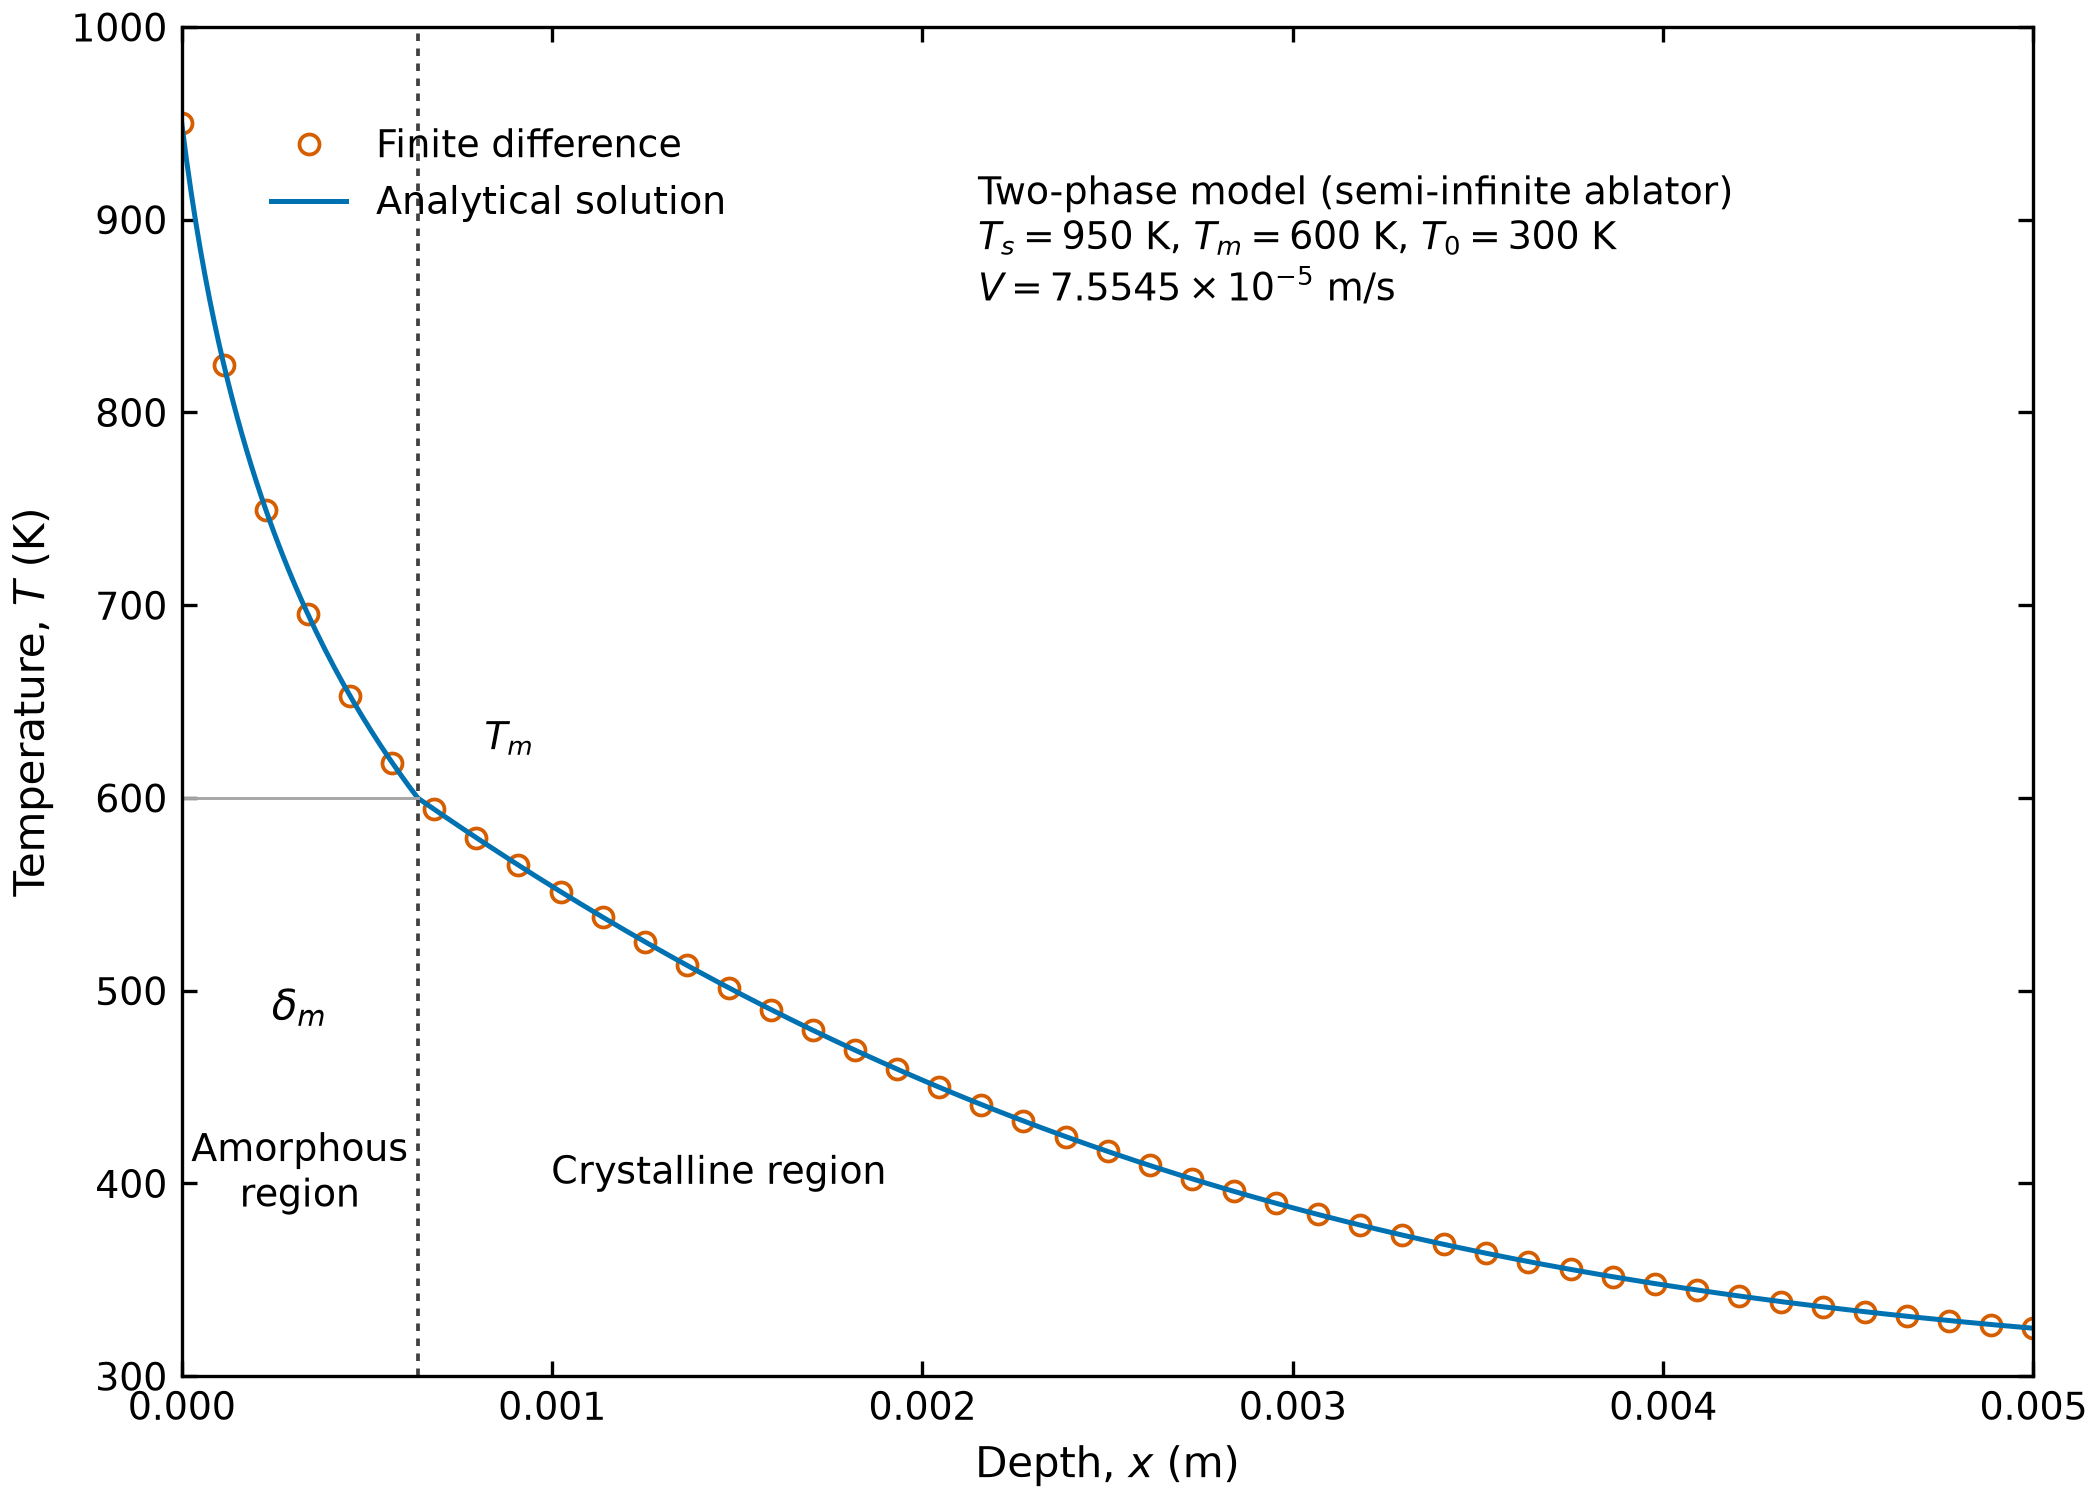
\includegraphics[width=\linewidth]{../plots/figure6.png}\\[-0.2em]
  {\small (a) Figure 6: analytical and finite-difference profiles.}
 \end{minipage}
 \hfill
 \begin{minipage}{0.49\linewidth}
  \centering
  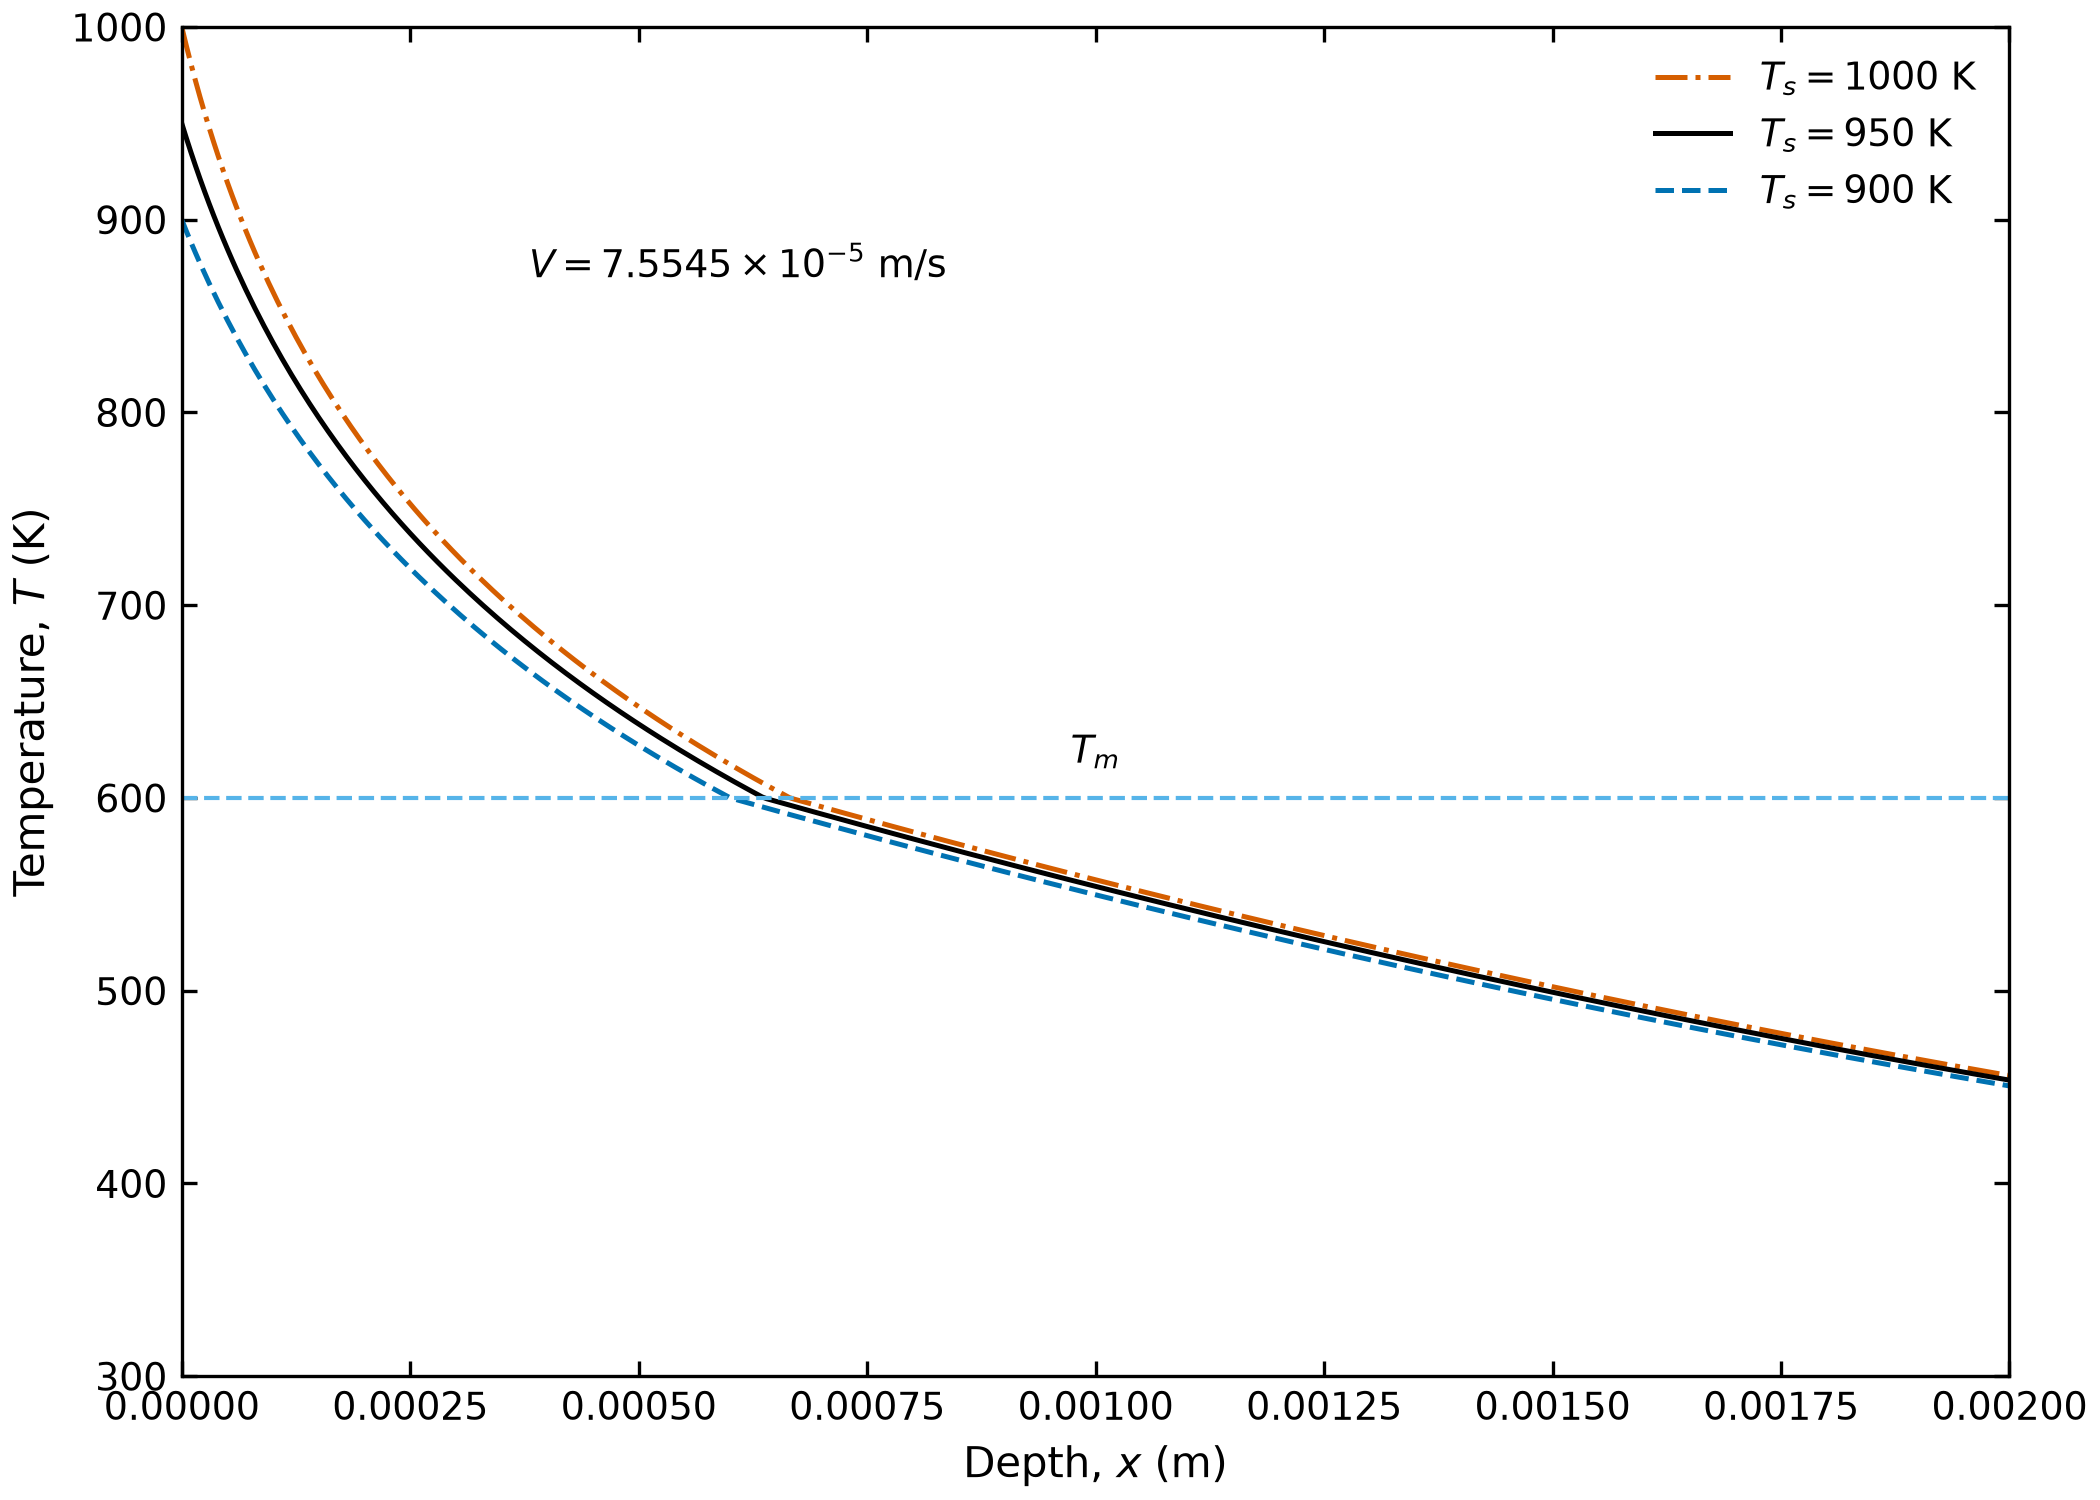
\includegraphics[width=\linewidth]{../plots/figure7.png}\\[-0.2em]
  {\small (b) Figure 7: surface-temperature sweep.}
 \end{minipage}
 \caption{Reproduced temperature profiles. Figure~6 compares the integral
 solution with the independent finite-difference result. Figure~7 changes
 $T_s$ while holding $V$ fixed.}
\end{figure}

\begin{figure}[htbp]
 \centering
 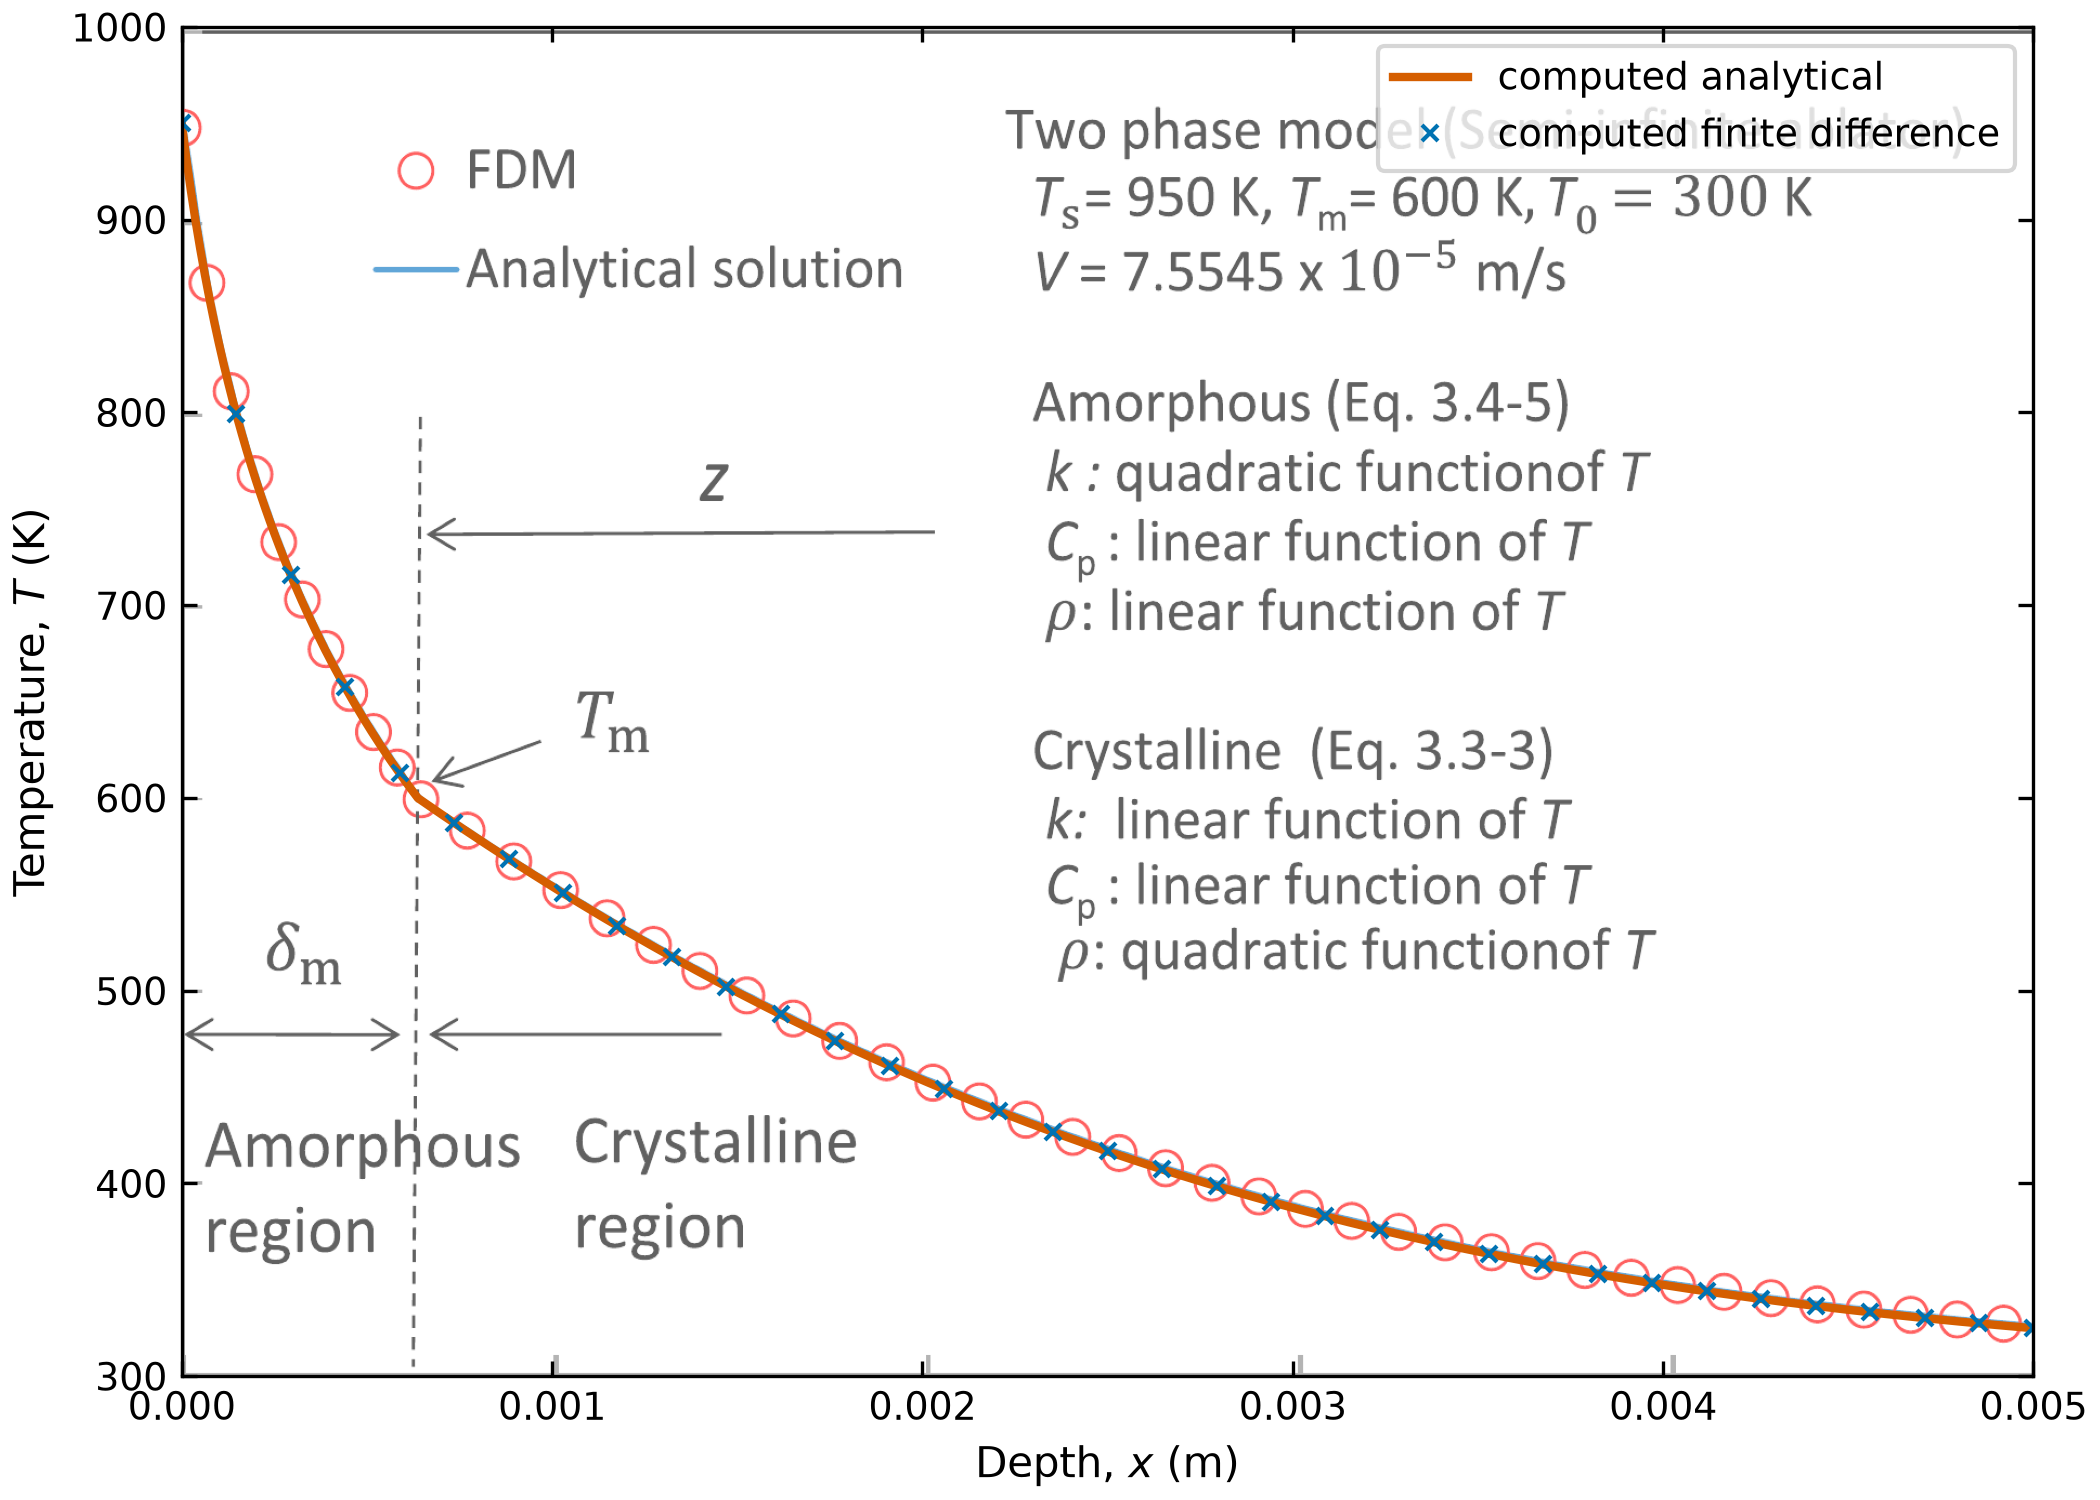
\includegraphics[width=0.70\linewidth]{../plots/figure6_overlay.png}\\[0.4em]
 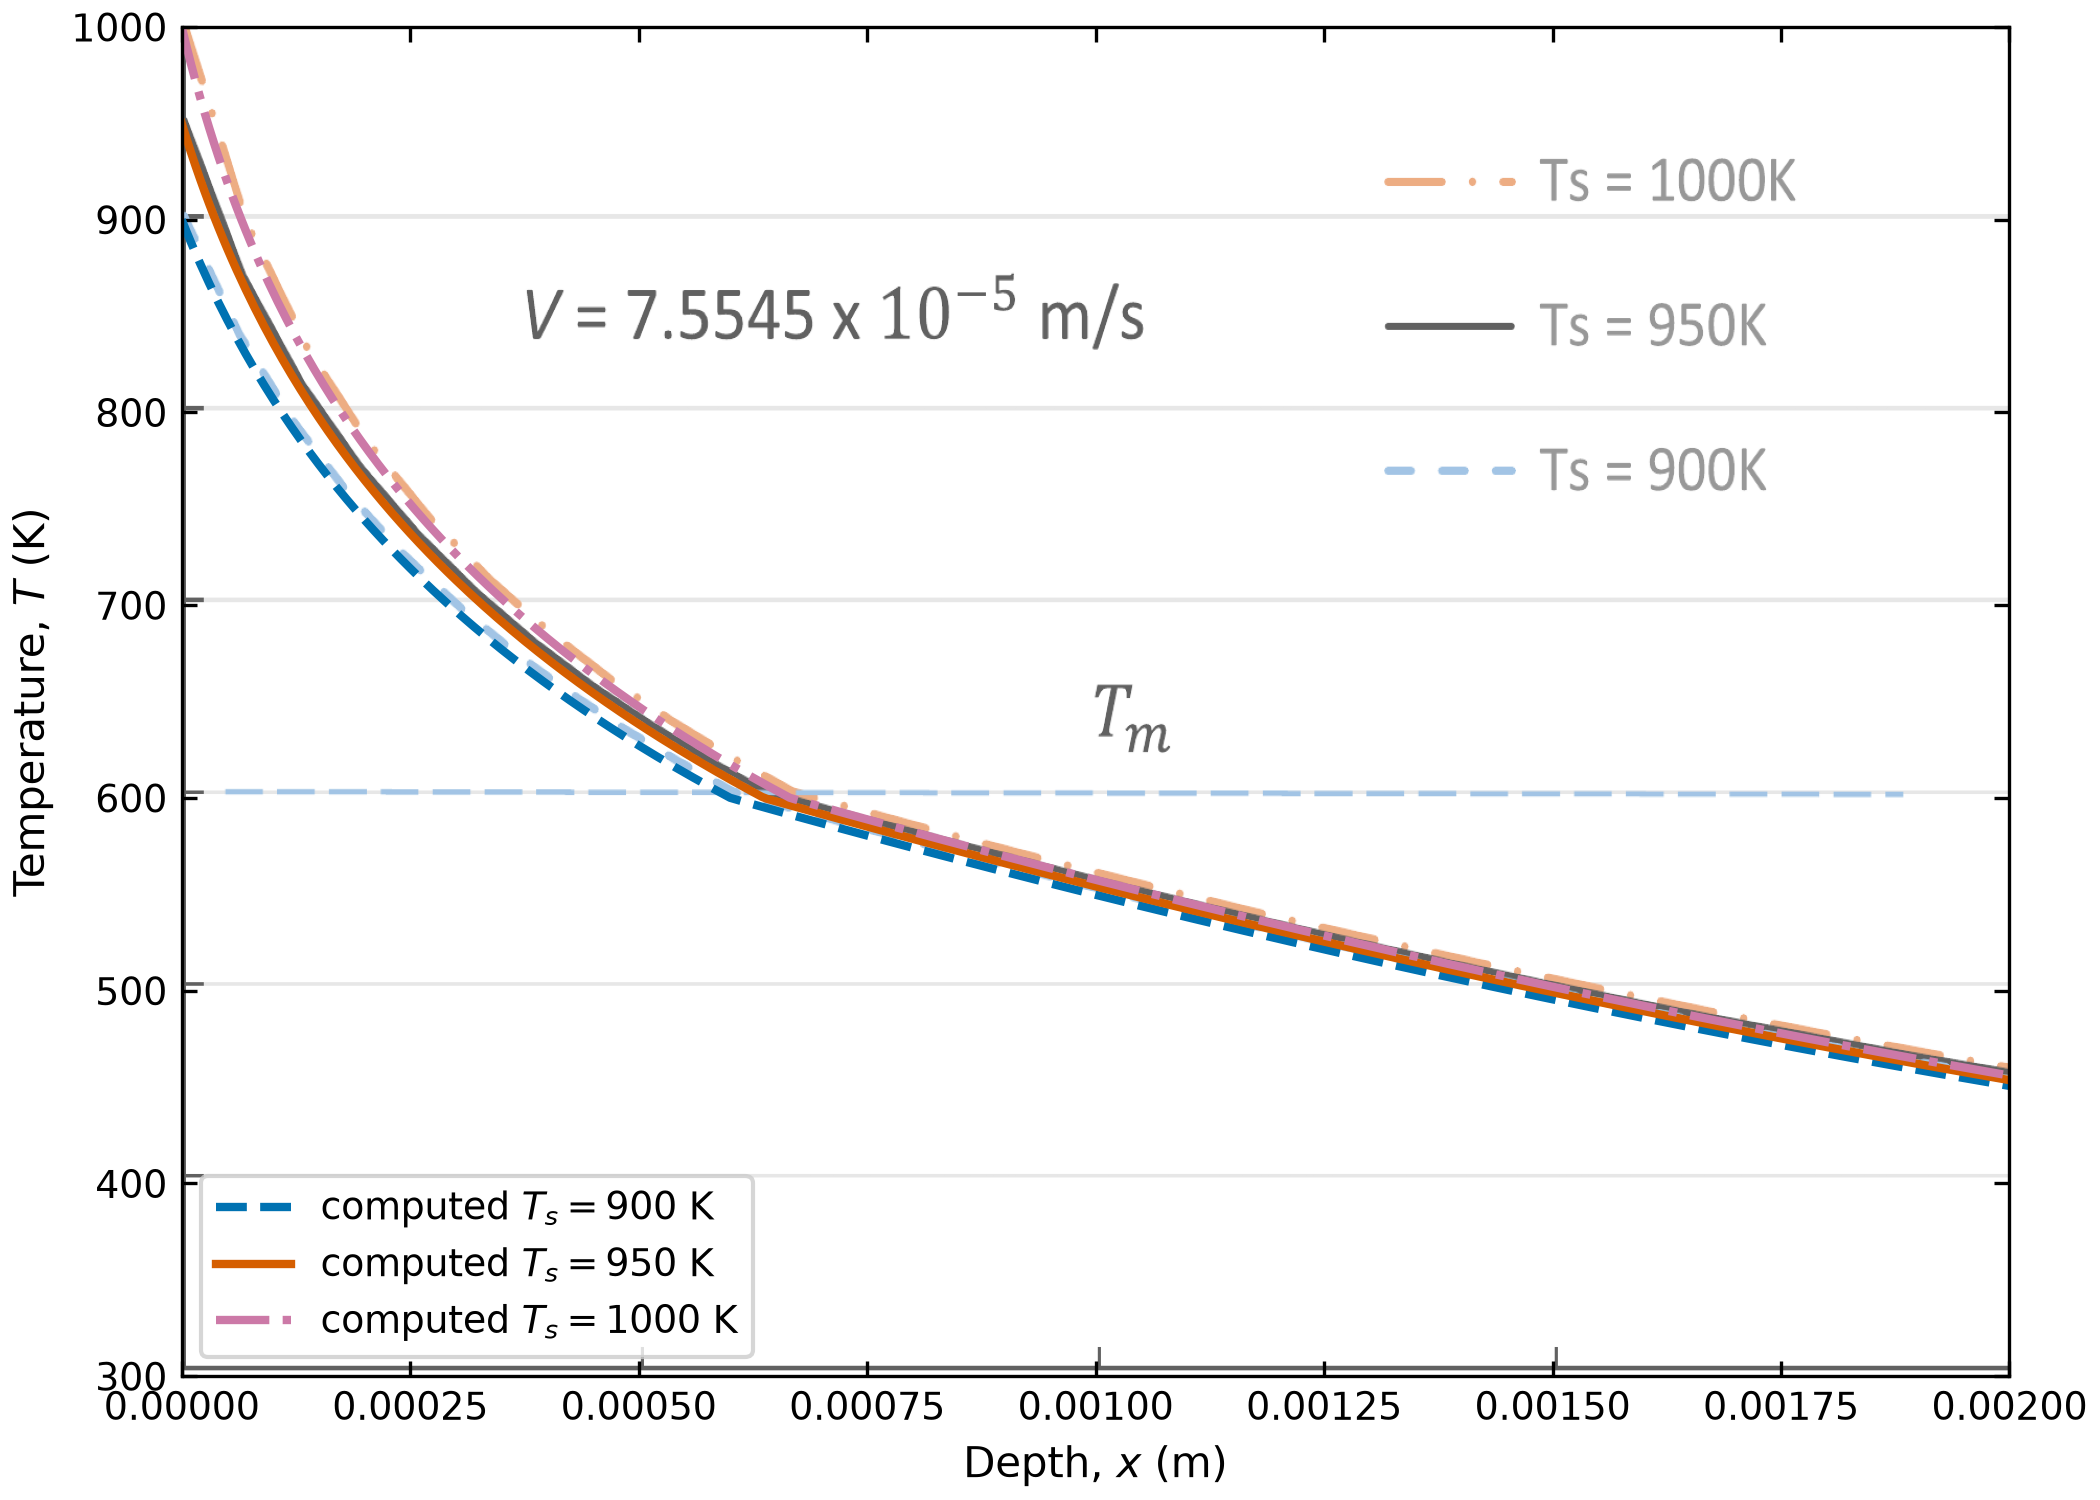
\includegraphics[width=0.70\linewidth]{../plots/figure7_overlay.png}
 \caption{Calculated profiles over the rasterized published Figures~6 and 7.
 The overlays check registration and curve shape. Numerical errors are
 calculated from the independent solutions, not from image pixels.}
\end{figure}

\clearpage
\section{Reproducibility}
From the project root, run
\begin{verbatim}
uv sync
uv run pytest
uv run python symbolic_derivation.py
uv run python compare_solutions.py
uv run python -m plots.plot_figure6
uv run python -m plots.plot_figure7
uv run python -m plots.plot_paper_overlays
cd writeup
latexmk -pdf -interaction=nonstopmode -halt-on-error derivation.tex
\end{verbatim}

\bibliographystyle{unsrt}
\bibliography{references}

\end{document}
